\documentclass[usenames,dvipsnames, 9pt]{beamer}
\usepackage{amsmath,amsfonts,amssymb}
\usepackage{mathtools}
\usepackage{etex} %for Windows
\usepackage[utf8]{inputenc}
\usepackage[english, russian]{babel} 
%\usepackage{microtype}			% Better interword spacing and additional kerning.
\usepackage{ellipsis}			% Adjusted space with \dots between two words.
\usepackage{graphicx}
\usepackage{pstricks}

\usepackage{xcolor}


\usepackage{changepage}

\usepackage{algorithm}
\usepackage{algpseudocode}
%\usepackage[]{algorithm2e}
%\usepackage{algorithmic}

%\usepackage{tcolorbox}






\usepackage{tikz}
\usetikzlibrary{tikzmark,calc}
\usetikzlibrary{positioning, backgrounds}
\usetikzlibrary{arrows, chains, matrix, scopes, patterns, shapes, fit}
\usetikzlibrary{mindmap,trees,shadows}
\usetikzlibrary{decorations.pathreplacing}
\usetikzlibrary{crypto.symbols}

\usepackage{pgfplots}

\pgfmathdeclarefunction{gauss}{2}{%
	\pgfmathparse{1/(#2*sqrt(2*pi))*exp(-((x-#1)^2)/(2*#2^2))}%
}


\tikzset{
	invisible/.style={opacity=0},
	visible on/.style={alt={#1{}{invisible}}},
	alt/.code args={<#1>#2#3}{%
		\alt<#1>{\pgfkeysalso{#2}}{\pgfkeysalso{#3}} % \pgfkeysalso doesn't change the path
	},
}

\newcommand\strikeout[2][]{%
	\begin{tabular}[b]{@{}c@{}} 
		\makebox(0,0)[cb]{{#1}} \\[-0.2\normalbaselineskip]
		\rlap{\color{Orange}\rule[0.5ex]{\widthof{#2}}{1.5pt}}#2
\end{tabular}}

\newcommand\Fontvi{\fontsize{11}{13.2}\selectfont}

\usepackage{listings} % for C++ code

\usepackage{braket}
%\usepackage[braket, qm]{qcircuit}



\usepackage[T1]{fontenc}
%\usepackage[sfdefault,scaled=.85]{FiraSans}
%\usepackage{newtxsf}
%\usepackage[nomap]{FiraMono}





\usefonttheme[onlymath]{serif}
\renewcommand\sfdefault{cmbr}

\renewcommand{\bfdefault}{sb}

\definecolor{CharCoalDark}{RGB}{13, 16, 19}
\definecolor{Orange}{RGB}{255, 165,0}
\definecolor{DarkOrange}{RGB}{255, 165,0}
\definecolor{LightSalmon}{RGB}{255, 160, 122}
\definecolor{LeafGreen}{RGB}{34, 139,  34}
\definecolor{Coral}{RGB}{255, 127, 80}
\definecolor{DarkTurquoise}{RGB}{0, 206, 209}

%\newtheorem{defRus}{Определение}
%\newtheorem{thmRus}{Теорема}
%s\newtheorem{corRus}{Следствие}


\setbeamercolor{background canvas}{bg=CharCoalDark}

\setbeamerfont{title}{series=\bfseries}
\setbeamercolor{title}{fg=Orange}
\setbeamercolor{section in toc}{fg=white}
\setbeamercolor{frametitle}{fg=Orange}
\setbeamercolor{normal text}{fg=white}
%\setbeamercolor{normal text}{fontsize=12pt}
\setbeamercolor{itemize item}{fg=Orange}
\setbeamercolor{enumerate item}{fg=Orange}
\setbeamercolor{enumerate item item}{fg=Orange}
\setbeamercolor{itemize item item}{fg=Orange}
\setbeamercolor{enumerate item}{fg=Orange}
\setbeamercolor{block title}{bg=DarkOrange,fg=white}
\setbeamerfont{block title}{series=\bfseries}

\setbeamertemplate{itemize item}[circle]
\setbeamertemplate{eumerate subitem}{\color{Orange}[$\checkmark$]}
\setbeamertemplate{itemize subitem}{\color{Orange}\Large$\textbullet$}
\setbeamertemplate{itemize subitem}{\color{Orange} \tiny $\blacksquare$}

% footnote without a marker
\newcommand\blfootnote[1]{%
	\begingroup
	\renewcommand\footnoterule{}
	\renewcommand\thefootnote{}\footnote{#1}%
	\addtocounter{footnote}{-1}%
	\endgroup
}

\newcommand*{\Scale}[2][4]{\scalebox{#1}{\ensuremath{#2}}}%

\newcommand\Item[1][]{%
	\ifx\relax#1\relax  \item \else \item[#1] \fi
	\abovedisplayskip=0pt\abovedisplayshortskip=0pt~\vspace*{-\baselineskip}}

\pgfdeclareradialshading{ring}{\pgfpoint{0cm}{0cm}}%
{rgb(0cm)=(1,1,1);
	rgb(0.7cm)=(1,1,1);
	rgb(0.719cm)=(1,1,1);
	rgb(0.72cm)=(0.975,0,0);
	rgb(0.9cm)=(1,1,1)}

\usepackage[absolute,overlay]{textpos} %to clip to a corner
\newcommand\FrameText[1]{%
	\begin{textblock*}{\paperwidth}(\textwidth-35pt, 10 pt)
		\raggedright #1\hspace{.5em}
\end{textblock*}}

\makeatletter
\let\save@measuring@true\measuring@true
\def\measuring@true{%
	\save@measuring@true
	\def\beamer@sortzero##1{\beamer@ifnextcharospec{\beamer@sortzeroread{##1}}{}}%
	\def\beamer@sortzeroread##1<##2>{}%
	\def\beamer@finalnospec{}%
}
\makeatother

\AtBeginSection[]
{
	\begin{frame}<beamer>
		\frametitle{Outline}
		\tableofcontents[currentsection]
	\end{frame}
}


%\institute{ENS Lyon}
\author{Elena Kirshanova \\ [10pt]
}
\titlegraphic{
	
	%\includegraphics[width=2.5cm]{erc_logo_gray}\hspace*{2.5cm}~%
	%\includegraphics[width=4.0cm]{ens_logo_gray}
}
\title{\Huge Block ciphers}

\date{ Course ``Information and Network Security'' \\ 	
	Lecture 3 \\ \today }


\setbeamertemplate{navigation symbols}{} %removes navigation

% proper highlightling of a code-snippet
\lstset{language=C++,
	keywordstyle=\color{magenta},
	stringstyle=\color{Goldenrod},
	commentstyle=\color{gray},
	breaklines=false,
	%morecomment=[l][\color{magenta}]{\#}
}

%\setlength{\parskip}{8pt}
% ==================================================================
% Definitions for this paper
% ==================================================================
\mathchardef\hyphen="2D

\usepackage{multirow}
\usepackage{multicol} % For multiple coloumn environments
%\usepackage{stmaryrd} % For set brackets
% \setlength{\columnsep}{15pt} % Defining the coloumn seperation
% \setlength{\columnseprule}{1pt} % Place a line between coloumns
% \newcommand{\tab}{\hspace*{2em}}

%subscripts

\newcommand*\SmallTextScript[2]{{\mathchoice{\displaystyle #2}
		{\textstyle #2}%dito
		{\scalebox{#1}{\ensuremath{\scriptstyle #2}}}%
		{\scalebox{#1}{\ensuremath{\scriptscriptstyle #2}}}%
}}


% ADVERSARIES AND SUCH
\newcommand*{\poly}{\ensuremath{\mathrm{poly}}}
\newcommand*{\eps}{\ensuremath{\varepsilon}}
\newcommand*{\alg}{\ensuremath{\mathcal{A}}}

% GROUPS/DISTRIBUTIONS/SETS/LISTS
\newcommand{\N}{{{\mathbb N}}}
\newcommand{\Z}{{{\mathbb Z}}}
\newcommand*{\IZ}{\ensuremath{\mathbb{Z}}}
\newcommand*{\IN}{\ensuremath{\mathbb{N}}}
\newcommand*{\IQ}{\ensuremath{\mathbb{Q}}}
\newcommand{\R}{{{\mathbb R}}}
\newcommand*{\IR}{{{\mathbb R}}}
\newcommand{\Zp}{\Z_p} % Integers modulo p
\newcommand{\Zq}{\Z_qs} % Integers modulo q
\newcommand{\Zn}{\ints_N} % Integers modulo N
\newcommand{\F}{\ensuremath{\mathbb{F}}}
\newcommand{\CC}{\ensuremath{\mathbb{C}}}

\newcommand{\ord}{\ensuremath{\mathrm{ord}}}

\newcommand{\GF}{\ensuremath{\mathbb{F}_2}}
\newcommand{\GFn}{\ensuremath{\mathbb{F}^n_2}}

%%% ALGORITHMS/PROCEDURES %%%
\newcommand{\Dec}{\textsf{Dec}}
\newcommand{\Enc}{\textsf{Enc}}
\newcommand{\KeyGen}{\textsf{KeyGen}}
\newcommand{\Gen}{\textsf{Gen}}
\newcommand{\MAC}{\textsf{MAC}}
\newcommand{\sk}{\textsf{sk}}
\newcommand{\pk}{\textsf{pk}}
\newcommand{\mesS}{\ensuremath{\mathcal{M}}}
\newcommand{\keyS}{\ensuremath{\mathcal{K}}}
\newcommand{\cipS}{\ensuremath{\mathcal{C}}}
\newcommand{\tagS}{\ensuremath{\mathcal{T}}}
\newcommand{\nonceS}{\ensuremath{\mathcal{N}}}
\newcommand{\mactag}{\textsf{tag}}
\newcommand{\Hash}{\ensuremath{\mathcal{H}}}
\newcommand{\EID}{\ensuremath{\mathtt{EphID}}}

\newcommand{\rem}{\ensuremath{\mathrm{rem}}}

\newcommand{\adv}{\ensuremath{\mathcal{A}}}

\newcommand{\LWE}{\mathsf{LWE}}
\newcommand{\DCP}{\mathsf{DCP}}
\newcommand{\EDCP}{\mathsf{EDCP}}
\newcommand{\UEDCP}{\mathsf{U \text{-} EDCP}}
\newcommand{\GEDCP}{\mathsf{G \text{-} EDCP}}



%% Landau and proba
\newcommand{\bigO}{\mathcal{O}}
\newcommand*{\OLandau}{\bigO}
\newcommand*{\WLandau}{\Omega}
\newcommand*{\xOLandau}{\widetilde{\OLandau}}
\newcommand*{\xWLandau}{\widetilde{\WLandau}}
\newcommand*{\TLandau}{\Theta}
\newcommand*{\xTLandau}{\widetilde{\TLandau}}
\newcommand{\smallo}{o} %technically, an omicron
\newcommand{\wLandau}{\omega}
\newcommand{\negl}{\mathrm{negl}}
\newcommand*\PROB\Pr 
\DeclareMathOperator*{\EXPECT}{\mathbb{E}}
\DeclareMathOperator*{\VARIANCE}{\mathbb{V}}
\DeclareMathOperator*{\LOGBIAS}{\mathbb{LB}}

\newcommand{\supp}{\ensuremath{\mathsf{sup}}}
\newcommand{\Distr}{\ensuremath{\mathcal{D}}}

% Lattices

% \newcommand{\coset}{\Lambda} % Lambda Lattice
% \newcommand{\cosetPerp}{\Lambda^{\bot}} % Lambda_Perp Lattice
% \newcommand{\gadget}{\textbf{G}} %Gaget matrix
% \newcommand{\mes}{\textbf{m}} %message vector
% \newcommand{\AMat}{\textbf{A}} %A matrices
% \newcommand{\BMat}{\textbf{B}} %B matrices
% \newcommand{\RMat}{\textbf{R}} %R matrices
% \newcommand{\HMat}{\textbf{H}} %H matrices
% \newcommand{\XMat}{\textbf{X}} %H matrices
% \newcommand{\mbar}{\bar{m}} %mBar dimension
% % \newcommand{\gauss}{\mathcal{D}} % gaussian distribution
% \newcommand{\Id}{\textbf{I}} % Identity matrix
% \newcommand{\er}{\textbf{e}} % gaussian distr. vectors
% % \newcommand{\cipher}{\textit{c}} % ciphertext
% \newcommand{\Olwe}{\mathcal{O}_{\textsf{LWE}}} %LWE oracle
% \newcommand{\OSample}{\mathcal{O}_{Sample}} %LWE oracle
% \newcommand{\SigmaB}{\boldsymbol{\Sigma}} %semi-deifinite matrix Sigma%
% % \newcommand{\mods}{\text{ mod}}


%Vectors and Matrices

\newcommand{\AMat}{\mathbf{A}} %A matrices
\newcommand{\BMat}{\mathbf{B}} %B matrices
\newcommand{\DMat}{\mathbf{D}} %Diagonal


\newcommand{\HMat}{\ensuremath{\mathbf{H}}}
\newcommand{\QMat}{\ensuremath{\mathbf{Q}}}
\newcommand{\Id}{\ensuremath{\mathbf{I}}}
\newcommand{\ZeroM}{\textbf{0}} % Zero matrix

\newcommand{\avec}{\ensuremath{\mathbf{a}}}
\newcommand{\bvec}{\ensuremath{\mathbf{b}}}
\newcommand{\cvec}{\ensuremath{\mathbf{c}}}
\newcommand{\evec}{\ensuremath{\mathbf{e}}}
\newcommand{\rvec}{\ensuremath{\mathbf{r}}}
\newcommand{\svec}{\ensuremath{\mathbf{s}}}
\newcommand{\tvec}{\ensuremath{\mathbf{t}}}
\newcommand{\vvec}{\ensuremath{\mathbf{v}}}
\newcommand{\zvec}{\ensuremath{\mathbf{z}}}
\newcommand{\xvec}{\ensuremath{\mathbf{x}}}
\newcommand{\yvec}{\ensuremath{\mathbf{y}}}
\newcommand{\uvec}{\ensuremath{\mathbf{u}}}
\newcommand{\zerovec}{\ensuremath{\mathbf{0}}}

\newcommand{\nth}{^{\mathrm{th}}}
\newcommand{\nd}{^{\mathrm{nd}}}

\newcommand{\RepMMT}{\ensuremath{\mathcal{R}_{\protect\SmallTextScript{0.70}{\texttt{MMT}}}}}
\newcommand{\RepBJMM}{\ensuremath{\mathcal{R}_{\protect\SmallTextScript{0.70}{\texttt{BJMM}}}}}
\newcommand{\XOR}{\ensuremath{\mathtt{3XOR}}}


% % % % % \newcommand{\mb}[1]{\mathbf{#1}} % does not compile otherwise
%%% Removed by Gotti; this is just asking to screw up with packages that (properly) define \mb (mathbold)

% \newcommand{\bL}{\|\bvec_1\|} % b1 length that appears way too often
% \newcommand{\dL}{\|\dvec_1\|} % b1 length that appears way too oftend

%Norms and Scalar products

\newcommand*\abs[1]{\left\lvert#1\right\rvert}
\newcommand*\norm[1]{\left\lVert#1\right\rVert}
\newcommand*\normalabs[1]{\lvert#1\rvert} 
\newcommand*\normalnorm[1]{\lVert#1\rVert}
\newcommand*\bignorm[1]{\bigl\lVert#1\bigr\rVert}
\newcommand*\bigabs[1]{\bigl\lvert#1\bigr\rvert}
\newcommand*\Bigabs[1]{\Bigl\lvert#1\Bigr\rvert}
\newcommand*{\ScProd}[2]{\ensuremath{\langle#1\mathbin{,}#2\rangle}} %Scalar Product
% \newcommand*{\ScProd}[2]{\ensuremath{\langle#1 \:{,}\:#2\rangle}} %Scalar Product
\newcommand*{\bigScProd}[2]{\ensuremath{\bigl\langle#1\mathbin{,}#2\bigr\rangle}} %Scalar Product
\newcommand*{\BigScProd}[2]{\ensuremath{\Bigl\langle#1\mathbin{,}#2\Bigr\rangle}} %Scalar Product
\newcommand{\dist}{\ensuremath{\text{dist}}}


%Some other math operators

\DeclareMathOperator{\Span}{Span} %span of vectors
\DeclareMathOperator{\vol}{\mathrm{vol}} %volume
\DeclareMathOperator{\LW}{LambertW} %Lambert W function
\DeclareMathOperator{\SD}{SD}
\DeclareMathOperator{\gradient}{grad}
\DeclareMathOperator{\TRACE}{Tr}
\newcommand*{\dDR}{\mathrm{d}} %de-Rham-Differential (the d in dx, dy, dz and so on)


%Lists
\renewcommand{\L}{\ensuremath{\mathcal{L}}}

\renewcommand{\P}{\ensuremath{\mathcal{P}}}

\newcommand*{\Lout}{\ensuremath{\L_{\mkern-0.5mu\protect\SmallTextScript{0.85}{\textup{out}}}}}
\newcommand*{\Sout}{\ensuremath{S_{\mkern-0.5mu\protect\SmallTextScript{0.85}{\textup{out}}}}}
\newcommand{\wt}{\ensuremath{\mathit{wt}}}


\newcommand*{\softO}{\widetilde{\bigO}}

\newcommand{\const}{\mathsf{c}} 


\newcommand{\transpose}{\mkern0.7mu^{\mathsf{ t}}}

%proper overline reduced by 1.5mu
\newcommand{\overbar}[1]{\mkern 1.5mu\overline{\mkern-1.5mu#1\mkern-1.5mu}\mkern 1.5mu}

\DeclareMathOperator{\erf}{erf} %error function
\DeclareMathOperator{\erfc}{erfc} %complementary error function
\newcommand{\Er}{\ensuremath{\mathrm{Er}}} %complementary error function


% LATTICES

\newcommand{\Lat}{\ensuremath{\mathcal{L}}}
\newcommand*{\Sphere}[1]{\ensuremath{\mathsf{S}^{#1}}}
%\DeclareMathOperator{\Conf}{Conf}
\newcommand{\Conf}{\mathcal{C}}

%Thick line for table
\setlength{\doublerulesep}{0pt}
\newcommand{\thickline}{\hline\hline\hline}


%circled text
\newcommand*\circled[1]{\tikz[baseline=(char.base)]{
    \node[shape=circle,draw,inner sep=0.3 pt] (char) {\scriptsize #1};}}


%Fix Algorithmicx package
\def\NoNumber#1{{\def\alglinenumber##1{}\State #1}\addtocounter{ALG@line}{-1}}

%For comments
\newcommand{\GColor}{ForestGreen}  %Damiens' color
\newcommand{\EColor}{MidnightBlue} %Elena's color

\newcommand*{\E}[1]{{\color{\EColor} #1} } 
\newcommand*{\G}[1]{{\color{\GColor} #1} } 

%Proper limit with the subscript underneath
% \newcommand{\Lim}[1]{\raisebox{0.5ex}{\scalebox{0.8}{$\displaystyle \lim_{#1}\;$}}}


%TIKZ dense dotted pattern

\pgfdeclarepatternformonly{my dots}{\pgfqpoint{-1pt}{-1pt}}{\pgfqpoint{2.0pt}{2.0pt}}{\pgfqpoint{2pt}{2pt}}%
{
	\pgfpathcircle{\pgfqpoint{0pt}{0pt}}{.35pt}
	\pgfpathcircle{\pgfqpoint{1pt}{1pt}}{.35pt}
	\pgfusepath{fill}
}


\tikzset{
	master/.style={
		execute at end picture={
			\coordinate (lower right) at (current bounding box.south east);
			\coordinate (upper left) at (current bounding box.north west);
		}
	},
	slave/.style={
		execute at end picture={
			\pgfresetboundingbox
			\path  (lower right)rectangle (upper left) ;
		}
	}
} %all defs
\begin{document}
	
\begin{frame}
	\titlepage
\end{frame}


\begin{frame}{Recap: PRG}
\LARGE 

\begin{itemize}
\itemsep1em

\item `Random' in crypto may come from two sources:

\begin{itemize}
	\item A `true' random number generator (or entropy generator) 
	\item An algorithmic ‘pseudorandom number generator’ (PRNG) 
\end{itemize}

\item 	{\color{Orange}\textbf{Pseudorandom generator (PRG)}} -- efficient algorithm taking on input truly random bits (seem) and outputting bits that are indistinguishable from random by ppt adversaries 

\item Examples: in Linux: $\mathsf{/dev/random},\mathsf{/dev/urandom}$ (not recommended for crypto applications); both use the same PRG (SHA-1); on Windows: CryptoAPI's  $\mathsf{CryptGenRandom}$

\item Better use established cryptographic PRGs, e.g.\ ChaCha, Salsa, HMAC-SHA1 or CBC-AES

\item Be aware of backdoored PRGs:  Dual EC DRBG
\end{itemize}

\end{frame}

\begin{frame}{Recap: PRG}
\LARGE 

\begin{itemize}
	\itemsep1em
	\item Statistical Tests: Diehard, NIST’s SP 800-22
	\item Known Answer Tests : BETTER NOT IN CODE RELEASE
\end{itemize}
\end{frame}

\begin{frame}{Recap: Stream ciphers}
	\LARGE 
	
	\begin{itemize}
		\itemsep1em
		\item Symmetric key is a seed to a PRG
		\item Encrypt:  $\Enc(m, s) = \mathsf{PRG}(s) \oplus m = c$ \\
				 Decrypt: $\Dec(c, s) = \mathsf{PRG}(s) \oplus c$
		\item ``Primitive''(=OTP) stream ciphers  are typically very fast and simple
		\item ... but inappropriate (=insecure) for many scenarios: broken by key re-use, require integrity checking
		\item Examples of practical stream ciphers: RC4, Trivium, A5/1 Generator
	\end{itemize}
\end{frame}

\begin{frame}{Block cipher}
\LARGE
	\begin{block}{Formal definition}
		A {\color{Orange}\textbf{Block cipher}} is a deterministic cipher with $\mathcal{X}:=\mesS = \cipS$ and a function
		\[
			f(k, \cdot): \mathcal{X} \rightarrow \mathcal{X}
		\]
	\end{block}
\begin{itemize}
	\item Correctness $\implies$ $f(k, \cdot)$ is one-to-one for all $k$. \\
	\item $|\mathcal{X}| < \infty$. \\
\end{itemize}

Thus, $f(k, \cdot)$ is a permutation on $\mathcal{X}$. \\[10pt]

{\color{Orange}\textbf{Security (informal) :}} $f(k, \cdot)$ ``looks like'' a random permutation 
\end{frame}

\begin{frame}{Block cipher in pictures}
		\begin{tikzpicture}
	%\draw[-stealth, thick] (-1.8,-1.0) -- (-1.0,-1.0) node[above,midway]{\Huge $b$};
	\draw[fill=CharCoalDark, draw=white, opacity=0.5] (-1.0,0.0) rectangle (2.0,1.0)  node[color=white, opacity=1,align=center, pos=0.5]{
		\LARGE  {Plaintext}  
	} node[above, midway, yshift=17pt]{\Large $n$ bits};
	\draw[-stealth, thick] (2.0,0.5) -- (3.0,0.5);

	\draw[fill=CharCoalDark, draw=white, opacity=0.5] (3.0,0.0) rectangle (5.0,1.0)  node[color=white, opacity=1,align=center, pos=0.5]{
		\LARGE  {$f, f^{-1}$}  
	};
	\draw[-stealth, thick] (5.0,0.5) -- (6.0,0.5);
	
	\draw[fill=CharCoalDark, draw=white, opacity=0.5] (2.5,2.2) rectangle (5.5,3.0)  node[color=white, opacity=1,align=center, pos=0.5]{
		\LARGE  {Key}  
	} node[above, midway, yshift=12pt]{\Large $k$ bits};

	\draw[-stealth, thick] (4.0,2.2) -- (4.0,1.0);
	
	\draw[fill=CharCoalDark, draw=white, opacity=0.5] (6.0,0.0) rectangle (9.0,1.0)  node[color=white, opacity=1,align=center, pos=0.5]{
		\LARGE  {Ciphertext}  
	} node[above, midway, yshift=17pt]{\Large $n$ bits};
	\end{tikzpicture}
	
	\vspace{15pt}
	\LARGE
	Examples:\\
	\begin{itemize}
		\item AES: $n = 128$, $k = 128, 192, 256$
		\item ГОСТ 34.12-2018: $n=128$, $k=256$ (Кузнечик)
	\end{itemize}
\end{frame}

\begin{frame}{A bit of history}
\Large
\begin{itemize}
	
	\itemsep1em
	\item {\color{Orange}\textbf{70's}:} IBM designs Lucifer. $k=128, n = 128$ 
	\item {\color{Orange}\textbf{'76}:} DES is standardised $k=56, n = 64$
	\item {\color{Orange}\textbf{'98}:} 3DES is standardised $k=168, n = 64$
	\item {\color{Orange}\textbf{'00}:} AES winner Rejndael $k=\{128, 192, 256\}, n = 128$
\end{itemize}

\vspace{10pt}
Russian standards:\\

\begin{itemize}
	
	\itemsep1em
	\item {\color{Orange}\textbf{'89}:} ГОСТ 28147-89 $k=256, n = 64$ 
	\item {\color{Orange}\textbf{'15 }:} ГОСТ Р 34.12-2015, RFC 7801 $k=256, n = 128$ 
\end{itemize}


\end{frame}

\begin{frame}{Block ciphers are iterative}
	\begin{figure}
		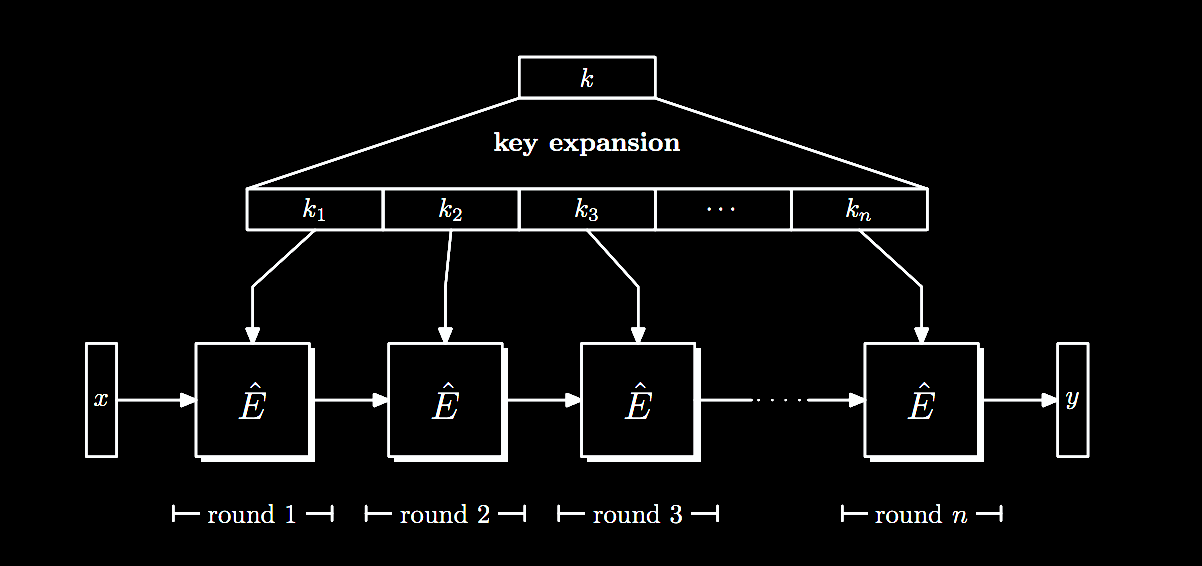
\includegraphics[width=1.1\textwidth]{BlockCipher}
	\end{figure}
	
	\Large 
	$x$ -- plaintext, $y$ -- ciphertext
	\vfill
	\small
	{\color{gray}\textbf{picture is taken from D.Boneh, V.Shoup A Graduate Course in Applied Cryptography}} 
\end{frame}

\begin{frame}{Two main paradigms in block cipher designs}

\begin{itemize}
	\itemsep 2em
	\LARGE
	\item Feistel cipher \\
	Сеть Фейстеля
	\\[5pt]
	
	\Large
	Examples: DES, ГОСТ 28147-89
	\LARGE
	\item Substitution-Permutation Network (SPN). \\ Подстановочно-перестановочная сеть  \\[5pt]
	\Large
	Examples: AES, ГОСТ 34.12-2018
	
\end{itemize}
\end{frame}

\begin{frame}{Feistel Cipher}
\Large
	Provides a generic way to build invertible functions from arbitrary functions. \\[10pt]
	Given \hspace{40pt} $f_1, \ldots, f_r: \{0,1\}^n \rightarrow \{0,1\}^n$ \\[7pt]
	construct an invertible $F:\{0,1\}^{2n} \rightarrow \{0,1\}^{2n}$ \\
	
	\vspace{20pt}
	\pause
	
	{\color{Orange}\textbf{Security (informal) :}} if $f: \keyS \times \{0,1\}^n \rightarrow \{0,1\}$ ``looks like'' a random function, then 3-Round Feistel $F: \keyS^3 \times \{0,1\}^{2n} \rightarrow \{0,1\}^{2n}$ is a pseudorandom permutation. 
\end{frame}


\begin{frame}{Example: GOST'89 Round function}
\centering
\tikzmark{start}
\includegraphics[height=0.85\textheight]{GostRound}
\tikzmark{end} 
\end{frame}

\begin{frame}{What's S-box?}
	\LARGE
	\[
		S:= \{0,1\}^n \rightarrow \{0,1\}^m
	\]

	\begin{itemize}
		\item Implemented as a look-up table
		\item There can be several S-boxes in one block-cipher
		\item Designed to be resistant to linear and differential cryptanalysis
		\item Must not contain any fixed points: \\ $S(x) \neq x $, $S(x) \neq  \bar{x} \; \forall x$
		\item S-box is {\color{Orange}\textbf{perfect}} if it's a \emph{bent} function (i.e., as ``far way'' from linear of affine boolean function as possible) 
	\end{itemize}
\end{frame}

\begin{frame}{Example: S-box in DES}
	\Large
	\[
	S:= \{0,1\}^6 \rightarrow \{0,1\}^4
	\]
	
	\begin{figure}
		\includegraphics[width=1.1\textwidth]{DES_Sbox}
			\hspace{2em}
	\end{figure}
\vfill
\small
{\color{gray} {picture taken from Wikipedia}} 
\end{frame}

\begin{frame}{Example: S-box in AES}
\Large
\[
S:= \{0,1\}^8 \rightarrow \{0,1\}^8
\]

\begin{figure}
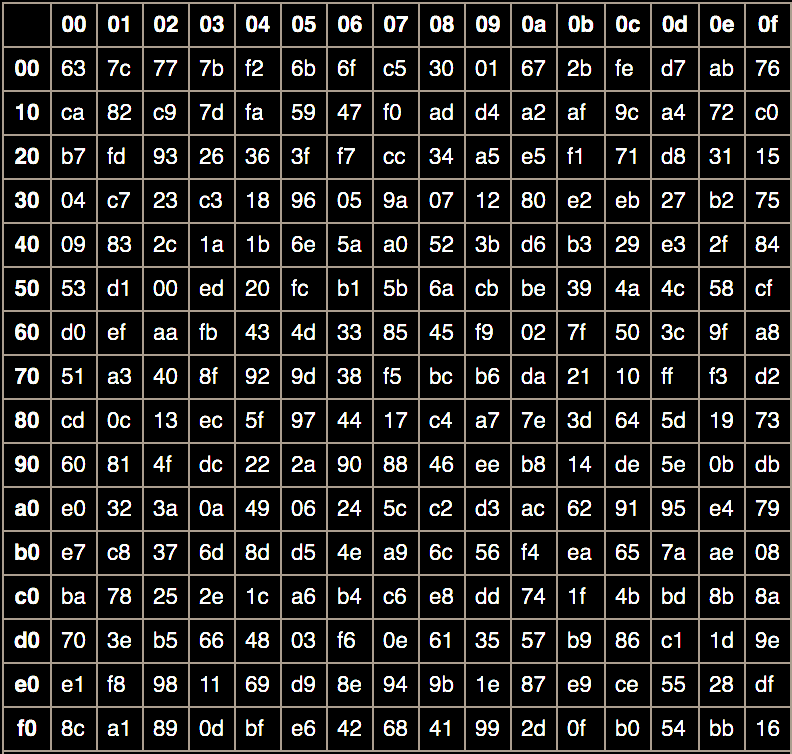
\includegraphics[width=0.7\textwidth]{AES_Sbox}
\end{figure}

\vfill
\small
{\color{gray} {picture taken from Wikipedia}} 

\end{frame}

\begin{frame}{Substitution-Permutation Network (SPN)}
\centering
\tikzmark{start}
\includegraphics[height=\textheight, angle=90, origin=c]{SPN}
\tikzmark{end} 

\end{frame}

\begin{frame}{AES: an SPN cipher}
	\begin{figure}
		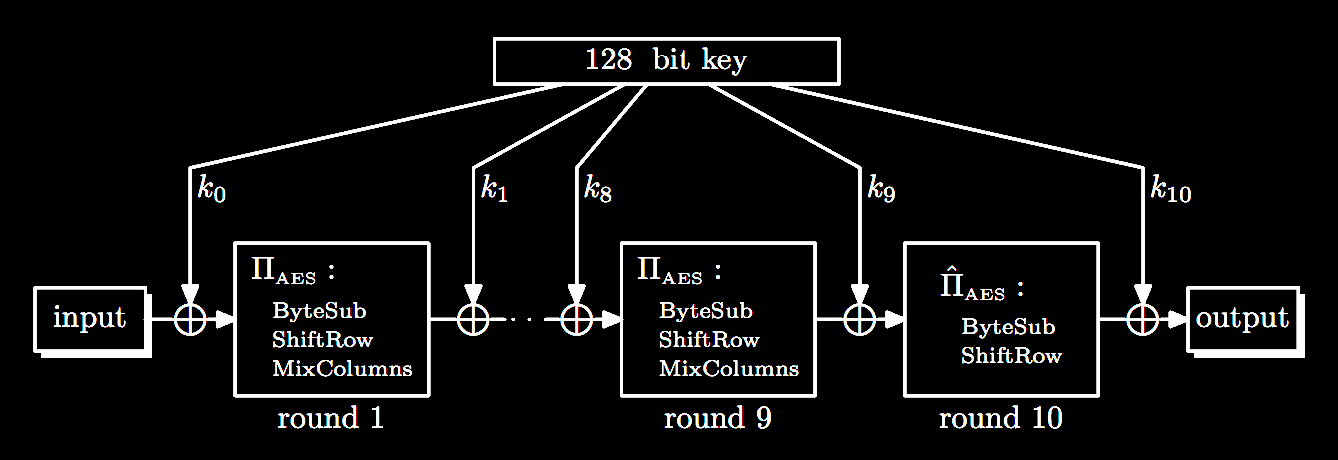
\includegraphics[width=1.1\textwidth]{AES_128}
	\end{figure}
	
	\Large 
	\[
		\Pi_{\text{AES}}  = \{0,1\}^{128} \rightarrow \{0,1\}^{128} - \text{ invertible permutation }
	\]
	\vfill
	\small
	{\color{gray}\textbf{picture is taken from D.Boneh, V.Shoup A Graduate Course in Applied Cryptography}} 
\end{frame}

\begin{frame}{Attacks on block ciphers}

\Large
{\color{Orange}\textbf{Exhaustive search}}  for block cipher key. \\[5pt]
	
	For DES/AES/GOST: \textbf{two} plaintext/ciphertext pairs $(m_1, c_1 = \Enc(k, m_1)), (m_2, c_2=\Enc(k,m_2))$ \\ determine $k$ with sufficiently high probability \\[10pt]
	
	
{\color{Orange}\textbf{Example}}  : For DES find $k \in \{0,1\}^{56}$	s.t.\ $c_i = \Enc(m_i, k)$. \\[10pt]

Cryptanalytic efforts: \\
\begin{itemize}
	\item {\color{Orange}\textbf{In '99}} ~22h on  DeepCrack + distributed.net (a bit expensive hardware)\\
	\item {\color{Orange}\textbf{In '07}}~13 days COPACOBANA (cheaper)
\end{itemize}
\end{frame}

\begin{frame}{Advanced attacks on block ciphers}
\LARGE
\begin{itemize}
	\itemsep 1em
	\item Design attacks: linear \& differential cryptnalalysis 
	
	Target:  find a linear relation in bit positions
	
	\begin{align*}
	& \Pr \left[ m[S_0] \oplus \Enc(k, m)[S_1 ] = k[S_2]  \right]  \geq 1/2 + \varepsilon  \\
	& S_i \subset \{0,\ldots, n-1\} \quad \forall k \text { and random } m
	\end{align*}
	\pause
	
	\item Side-channel attacks:
	\Large{measure {\color{Orange}\textbf{time}} or {\color{Orange}\textbf{power}} needed for  $\Enc, \Dec$ } \pause
	\LARGE
	\item Fault-injection attacks: 
	\Large cause the hardware to introduce errors at runtime (heat, EM interference)
\end{itemize}
\end{frame}

\begin{frame}{Take-home message}
\Huge

\begin{itemize}
	\itemsep 2em
	\item {\color{Orange}\textbf{DON'T}} design {\color{Orange}\textbf{YOUR OWN}} block-cipher 
	\item {\color{Orange}\textbf{TRY NOT TO}}  implement cryptoprimitives yourself if good implementations exist
	\item Choose key-sizes wisely 
\end{itemize}
\end{frame}


\begin{frame}{Further reading}
	\begin{figure}
		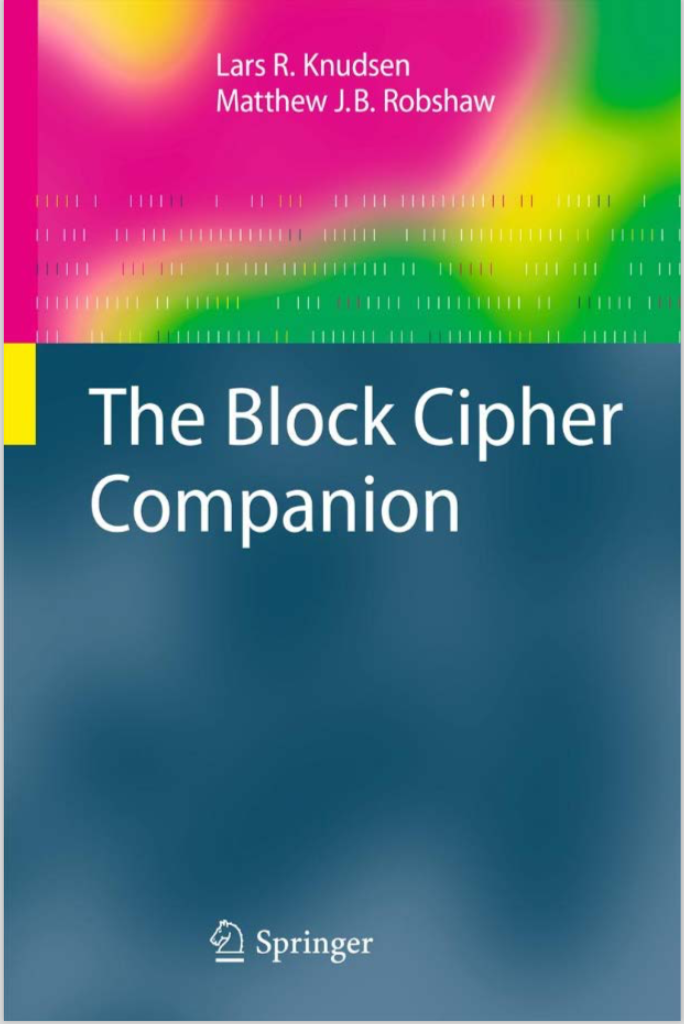
\includegraphics[height=0.7\textheight]{Book_cover}
	\end{figure}
\end{frame}

\end{document}